\documentclass{beamer}


\usetheme{light}


\title{Quasicrystals}
\subtitle{Physics 211 - Fall 2020}
\author{Eric Weise}
\date{}


\begin{document}

	\frame {
        \titlepage
	}

	\frame {
		\frametitle{Outline}
		\tableofcontents
	}




	\section[Section]{What is a Quasicrystal?}

    \frame {
        \frametitle{What is a Quasicrystal?}
        \framesubtitle{Ordered but not Periodic}

        \begin{itemize}
            \item Ordered: Constructed from a finite set of regular shapes.
            \item Not Periodic: Translational symmetry does not exist (but rotational symmetry does.)
        \end{itemize}
    }

    \frame {
        \frametitle{Penrose Tilings}
        \framesubtitle{Formalized Aperiodic Coverings of the 2D plane}

		\begin{columns}
		\column{0.4\textwidth}
            In 1974 Roger Penrose published his first aperiodic tiling of the 2D plane.
            It consisted of 6 repeating shapes, called prototiles.
		\column{0.6\textwidth}
            \centering
            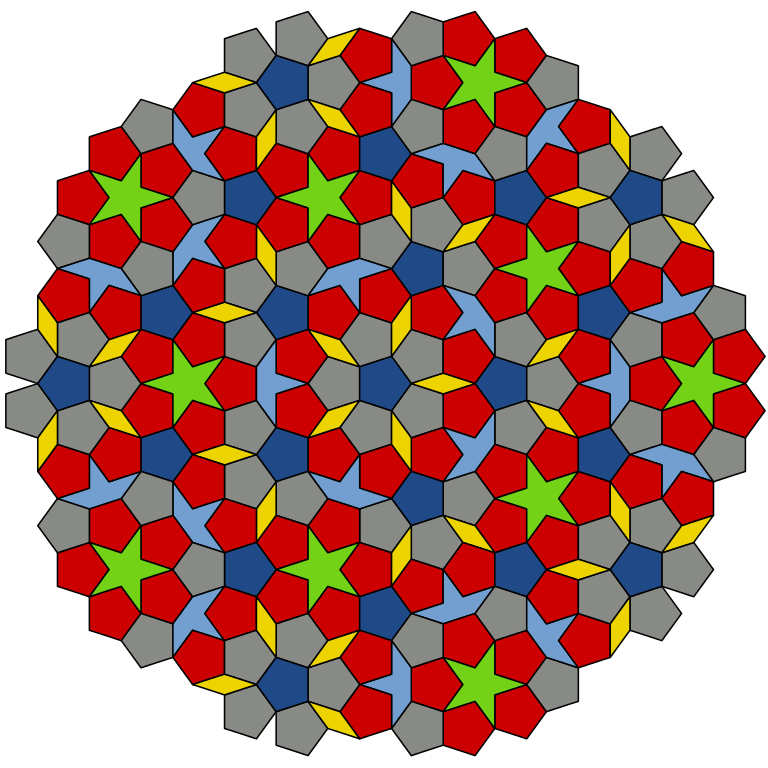
\includegraphics[keepaspectratio=true, width=0.6\textwidth]{images/penrose-p1.png}
		\end{columns}
    }

    \frame {
        \frametitle{Aeriodicity}
        \framesubtitle{An Informal Demonstration}

        \centering
        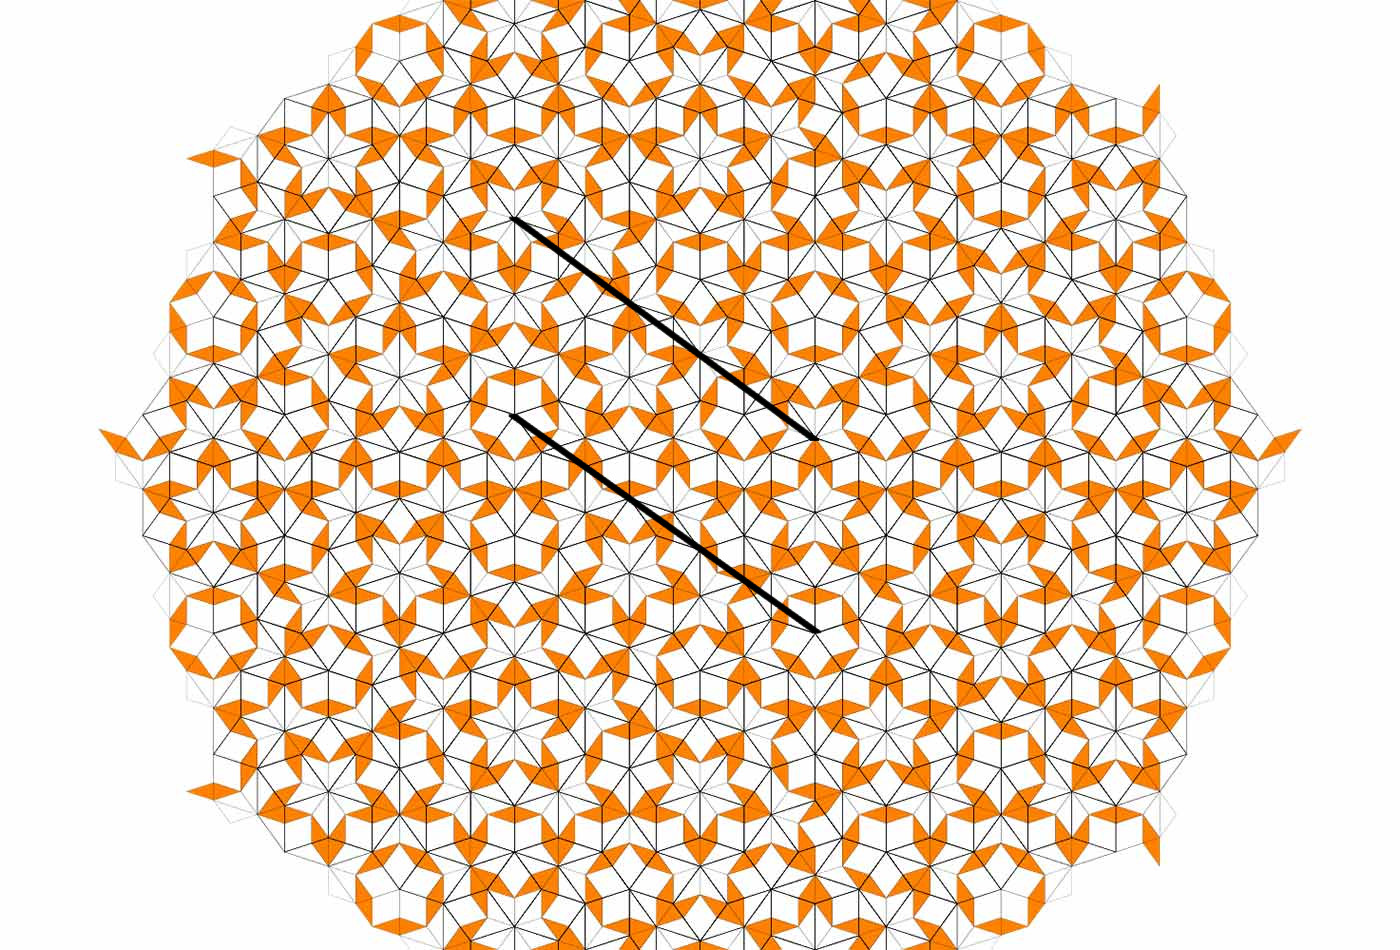
\includegraphics[keepaspectratio=true, height=0.75\textheight]{images/penrose-p3.jpg}
    }

    \frame {
        \frametitle{Aperiodicity}
        \framesubtitle{A slightly more rigorous approach}


        Prototiles in a Penrose tiling can be {\it deflated} into 
        prototiles of the same family, smaller by a constant factor. 
        This creates a fractal-like self similarity: extending the 
        tiling is the same as decomposing and scaling.

        \hspace{5px}

        \begin{columns}
        \column{0.5\textwidth}
            Start with a coarse aperiodic tiling.

            \centering
            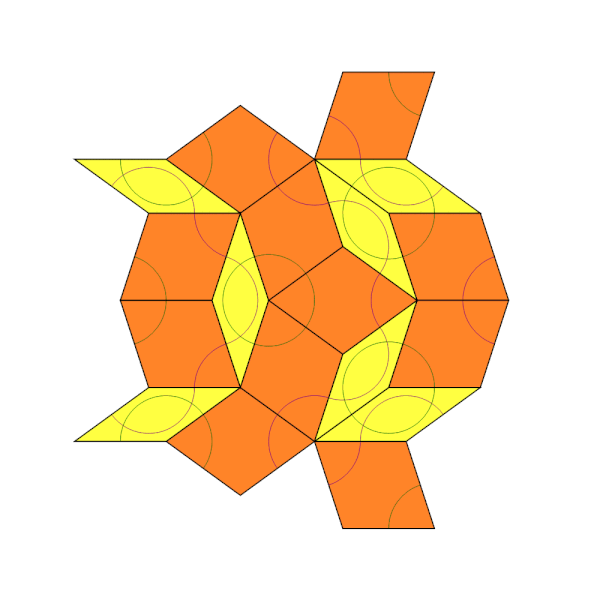
\includegraphics[keepaspectratio=true, width=0.33\textwidth]{images/deflation-1.png}

        \column{0.5\textwidth}
            Decomposing the tiling will not create any periodicity because
            the resulting pattern contains the same aperiodic pattern of
            the parent.

            \centering
            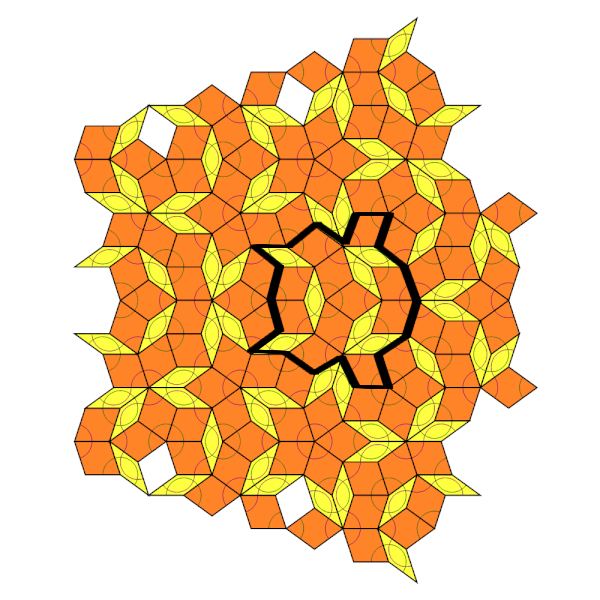
\includegraphics[keepaspectratio=true, width=0.33\textwidth]{images/deflation-2.png}
        \end{columns}

        \vspace{15pt}

        https://en.wikipedia.org/wiki/File:Penrose\_P3\_Deflations.gif

        % Think of it in reverse:
        % Assume there is a distance that is a translational symmetry, 
        %    and it exists within the right tiling.
        % we can INFLATE the tiling (combine the prototiles to make them larger)
        %    This should preserve the translational symmetry 
        %    BECAUSE the pattern is self similar
        % But, we can alwas inflate to a pattern that isn't periodic,
        %    LIKE the tiling on the left
    }

    \frame {
       \frametitle{``Forbidden Symmetries'' in 2D?}

        \centering
        \hbox{
            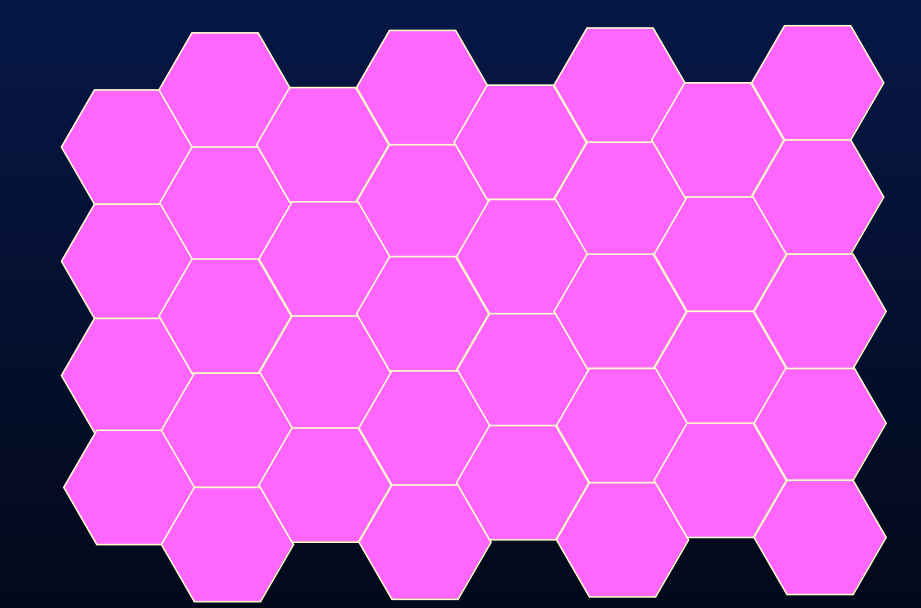
\includegraphics[keepaspectratio=true, width=0.35\paperwidth]{images/2d-sym-hex.png}
            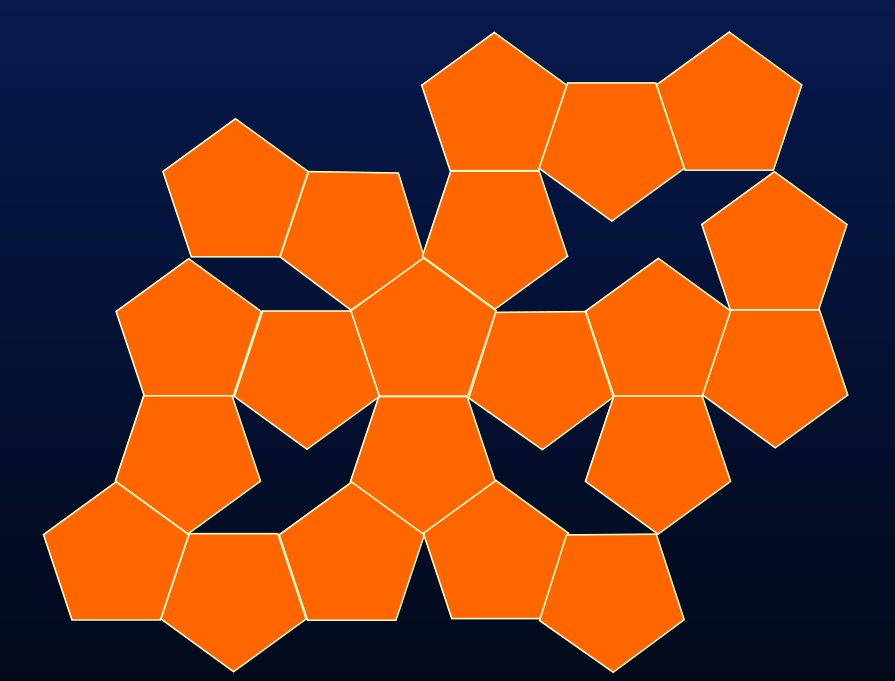
\includegraphics[keepaspectratio=true, width=0.35\paperwidth]{images/2d-asym-pent.png}
        }

        % While it is counterintuitive to imagine a 5-fold
        %   symmetry in 2D, we have shown that it is possible if we 
        %   forgo translational symmetry.

        % We will do the same for 3D.
    }


    \frame{
        \frametitle{The Isocahedron}
        \framesubtitle{A ``Forbidden Symmetry'' in Matter}

        \centering
        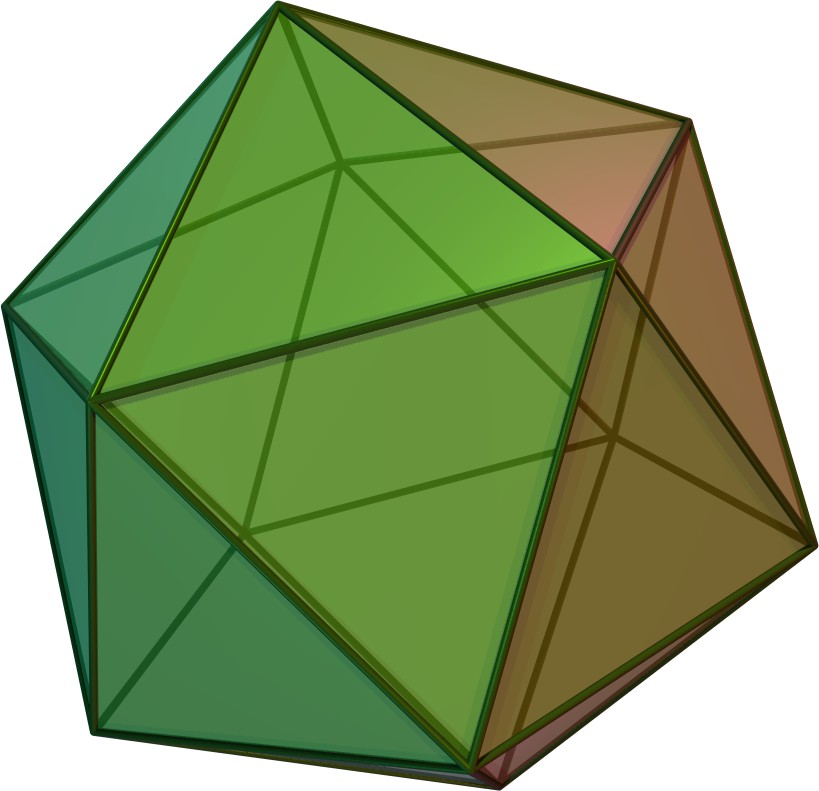
\includegraphics[keepaspectratio=true, height=0.35\textheight]{images/icosahedron.jpg}
        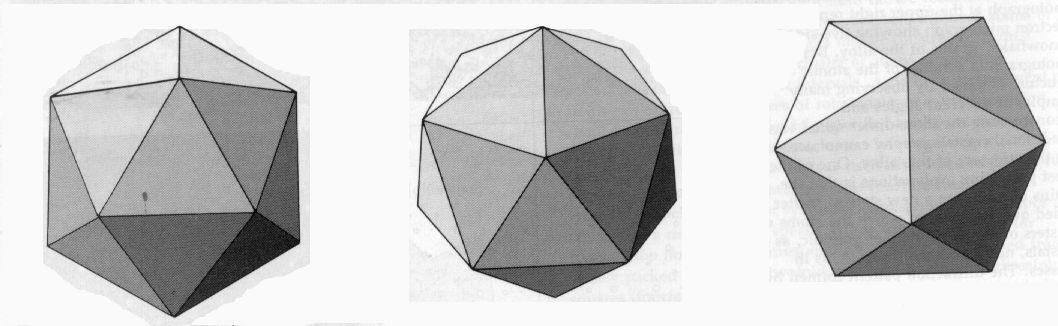
\includegraphics[keepaspectratio=true, height=0.35\textheight]{images/isocahedron-symmetries.png}

        % Note the 3- 5- and 2- fold symmetries

        % It is the 5-fold symmetry that we look for when we classify quasicrystals.

        % Forbidden because this shape cannot be made of smaller elements of itself. 
        % Therefore if it is made of a repeted pattern it must be a Quasicrystal.
    }








	\section[Section]{A Brief History}

    \frame{
        \frametitle{A Brief History of Quasicrystals}

        \begin{itemize}
            \item 1974: Sir Roger Penrose formalizes 2D aperiodic tilings
            \item 1981: Paul Steinhardt predicts existence of quasicrystals
            \item 1982: Daniel Shechtman discovers first quasicrystal in the lab
            \item 2007: Luca Bindi discovers first naturally formed quasicrystal
            \item 2011: Nobel Prize in Chemistry awarded to Daniel Shechtman
        \end{itemize}

    }

    \frame{
        \frametitle{Predicting the Existence of Quasicrystals}
        \framesubtitle{The Search is On}

        The existence of real quasicrystals was first predicted by Paul Steinardt in 1981.

        \vspace{15pt}

        \hbox{
            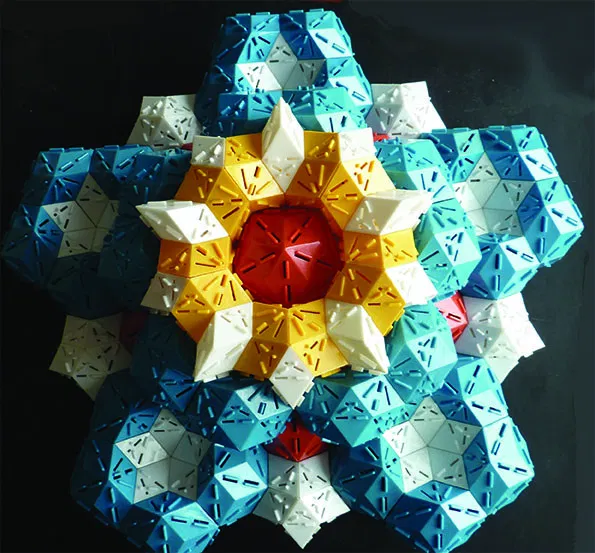
\includegraphics[keepaspectratio=true, height=4cm]{images/steinhart_quasicrystal_structure.png}
            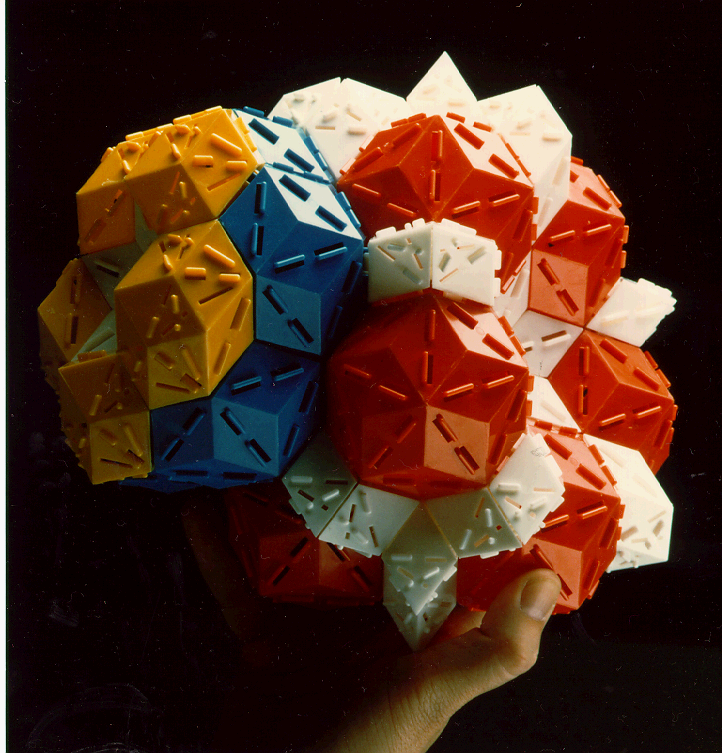
\includegraphics[keepaspectratio=true, height=4cm]{images/steinhart_quasicrystal_structure2.png}

            % Computer simulations showed their feasability under extremely quick cooling

            % He builds these elaborate models to help visualize the quasicrystals in 3D

            % These are the same crystal build out in different directions

            % See elements of the penrose tilings and the 5-fold symmetry
		}
    }

    \frame{
        \frametitle{First Detection}
        \framesubtitle{\(Al_6Mn\)}

		\begin{columns}
		\column{0.5\textwidth}
            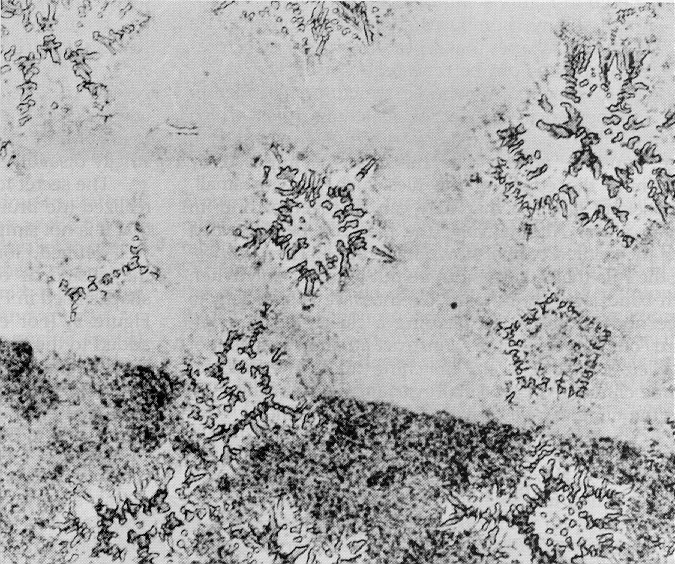
\includegraphics[keepaspectratio=true, height=0.35\textheight]{images/shechtman-realspace.png}
            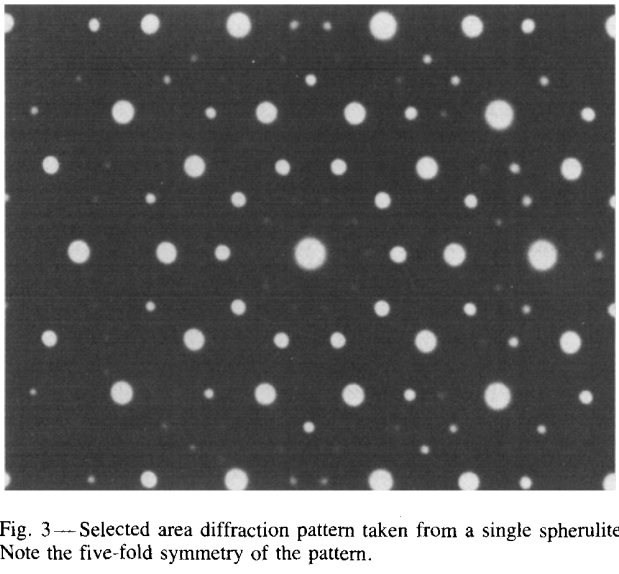
\includegraphics[keepaspectratio=true, height=0.35\textheight]{images/shechtman-diffraction.png}
		\column{0.5\textwidth}
            \begin{itemize}
                \item Discovered in 1982 by Dan Shechtman
                \item Verified in 1984 by Ilan Blech
                \item Evidence of isocahedral structure in matter
            \end{itemize}
		\end{columns}

        % Rapid cooling

        % Immediate controversy, Shechtman was ridiculed for jumping to conclusions

        % Was asked to leave the research group he was part of.

        % Easy to see how tiling of rectangular prisms can exist, but isocahedrons is counterintuitive.


        % Counterexamples:
        %    (1) A series of twinned microcrystals such as previously
        %    suggested for very thin gold films. 7'8'9
        %    (2) A layered twinned structure in which the twins are lay-
        %    ers rotated with respect to each other by 72 deg.
        %    (3) Five separate crystals enveloping each other (such as a
        %    helix with five branches).
        %    (4) A structure consisting of multiple polyhedra having lim-
        %    ited orientations.
    }

    \frame {
        \frametitle{Khatyrka Meteorite}
        \framesubtitle{Naturally Occuring Quasicrystals}

        In 2007 meteorologist Luca Bindi finally discovers Steinhart's 
        elusive sample in the Khatyrka meteorite.
        \vspace{15pt}

		\begin{columns}
		\column{0.5\textwidth}
            \centering
            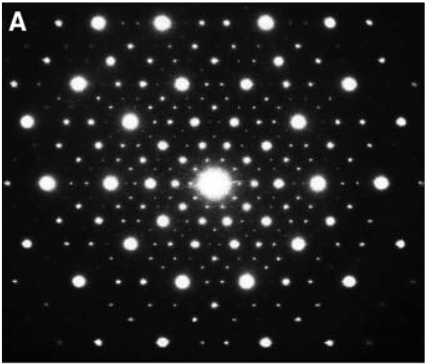
\includegraphics[keepaspectratio=true, height=4cm]{images/diffraction-meteor.png}

            Powder XRD pattern
		\column{0.5\textwidth}
            \centering
            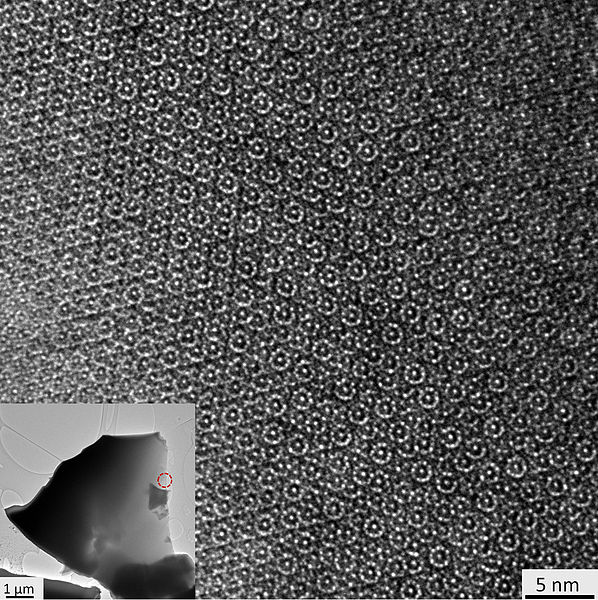
\includegraphics[keepaspectratio=true, height=4cm]{images/meteor-real.jpg}

            Magnified view of sample
		\end{columns}

        % Only three naturally occurring quasicrystals have been found, all from the same meteorite

        % found in Siberia
    }









	\section[Section]{Properties}

    \frame{
        \frametitle{General Characteristics}

        \begin{columns}
            \column{0.5\textwidth}
            \begin{itemize}
                \item Have at least one symmetry that is not 2- 3- 4- or 6-fold
                \item Exhibit rotational symmetry
                \item Grown under extreme cooling
                \item Usually (but not always) contain Aluminum
            \end{itemize}

            \column{0.5\textwidth}
            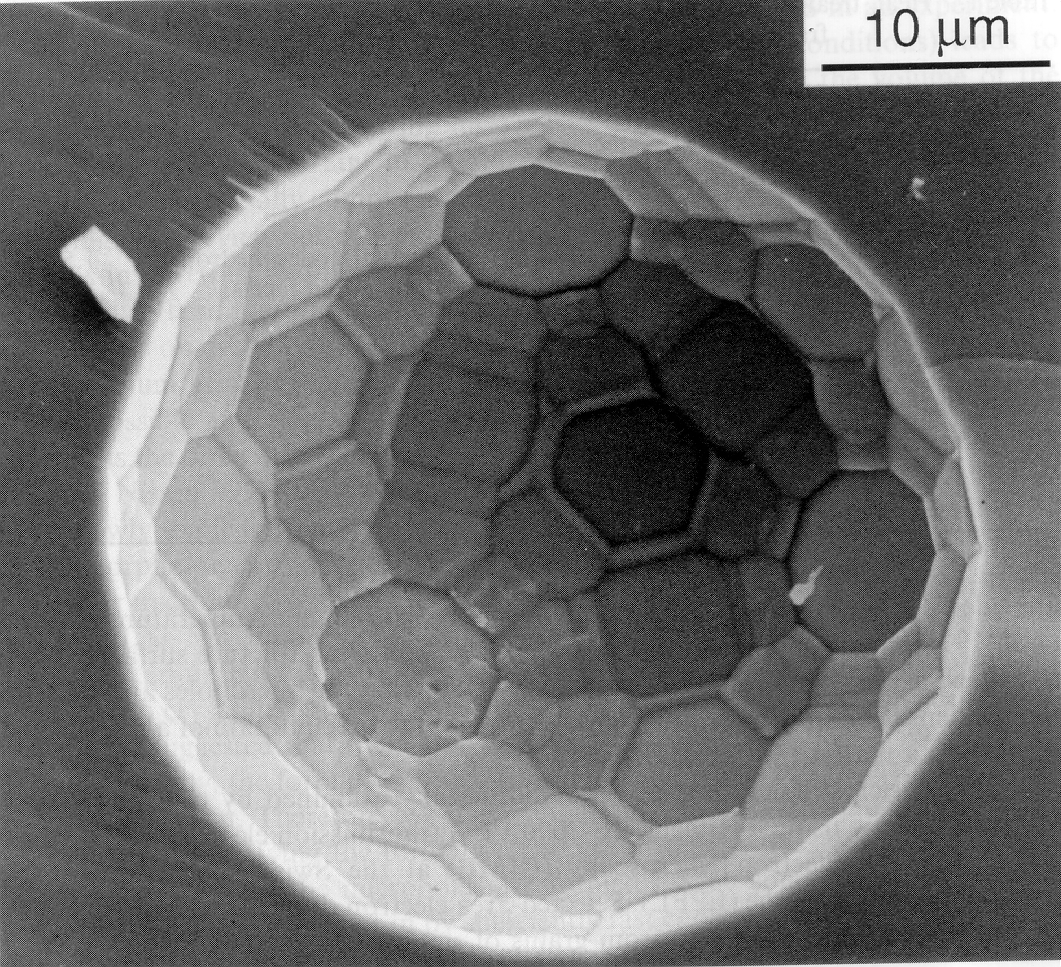
\includegraphics[keepaspectratio=true, width=5cm]{images/almnpd-crystal.png}

            AlMnPd
        \end{columns}
    }

    \frame{
        \frametitle{Classifying Quasicrystals}

        \centering
        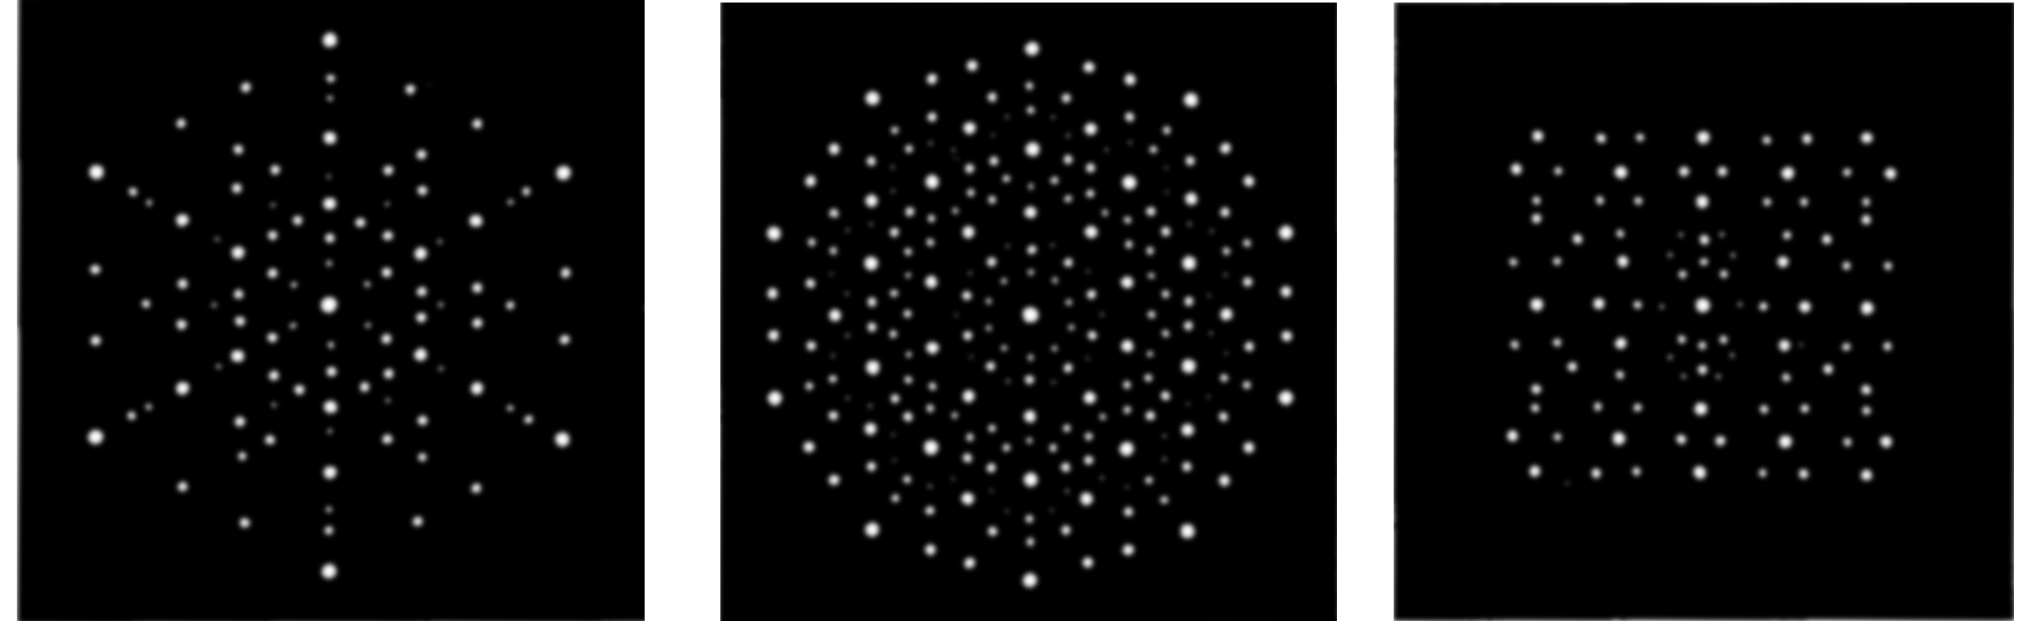
\includegraphics[keepaspectratio=true, height=0.35\paperheight]{images/diffraction-isocahedron-simulated.png}
        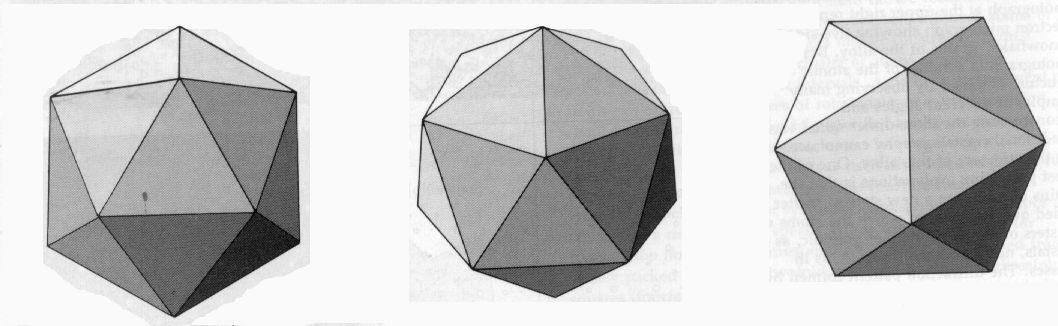
\includegraphics[keepaspectratio=true, height=0.35\paperheight]{images/isocahedron-symmetries.png}

        % Experimentally, the aperiodicity is revealed in the unusual symmetry of the diffraction pattern, that is, symmetry of orders other than two, three, four, or six
    }

    \frame{
        \frametitle{Electrical and Thermal Conductivity}

        Due to the lack of translational symmetry in quasicrystal 
        structures electron and phonon transport resembles that 
        of insulators for large energies.

        \vspace{15pt}

        \centering
        \hbox{
            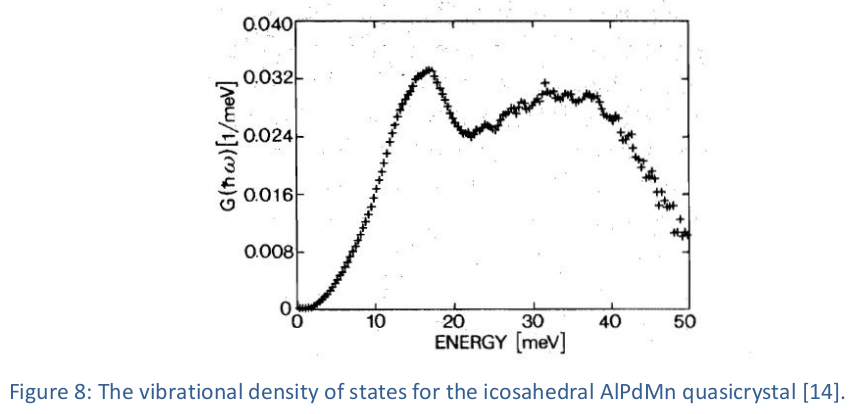
\includegraphics[keepaspectratio=true, height=0.35\paperheight]{images/phonon-dos.png}
            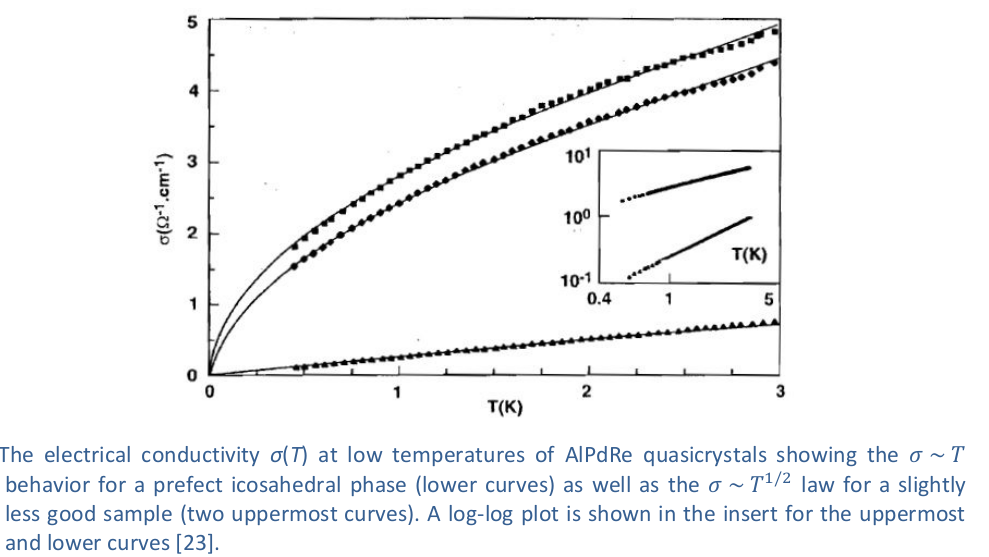
\includegraphics[keepaspectratio=true, height=0.35\paperheight]{images/conductivity.png}
        }

        \vspace{15pt}

        % The thermal
        %    conductivity values K(T) are indeed very small - much smaller than those expected for purely metallic
        %    compounds.
        % at room temperature, K(T) for quasicrystalline AlFeCu and AlPdMn is more
        %    than 100x smaller than for aluminium, 
        %    and 10x smaller than iron

        % At around 0.5K, the electrical resistivity of this QC can exceed 30Ωcm, a
        %    value which is 10^9 to 10^10 
        %    times larger than that of pure aluminium (Fig. 10.1)
    }








	\section[Section]{Applications}

    \frame{
        \frametitle{Applications}
        \begin{itemize}
            \item Thermoelectric power
            \item Energy coating for solar cells
            \item Phonon Bandgap Materials
            \item Surface coating
        \end{itemize}

        % Thermoelectric power coefficients up to several tens of μV/K
        % This effect can be used to accurately monitor a temperature
        %    setting without the help of sophisticated electronic devices.

        % electron-plasma oscillation a mean-free amplitude of about 22 Angstrom, 
        %    meaning optical conductivity peakes in the visual spectrum 
        %    when sandwiched between two oxide layers

        % low friction coefficient, high hardness, elevated corrosion resistance, a ductile-
        %    brittle transition, and superplasticity above 700C
        %    Great for coating stuff!
        %      razors, non-stick pans
    }






    \frame {
        \frametitle{Thank You}

        Thank you for listening!

        Questions?
    }

\end{document}
